%!TEX root = ../elaboration.tex
\chapter{System Proposal}
\label{cha:systemProposal}
%Descrição da arquitetura
%\begin{itemize}
%    \item Como recebemos dados dos IMU
%    \item Quando recebemos dados dos IMU (freq.)
%    \item 3 "Módulos" - Explicar cada um deles
%    \begin{enumerate}
%        \item Edge: sensores e raspberry Pi
%        \item Server
%        \item Client
%    \end{enumerate}
%    \item Comunicação entre os módulos
%\end{itemize}
%---------

\epigraph{
    To achieve the goals set in Chapter \ref{cha:introduction}, a system that collects and processes the raw data from the IMU sensors and transforms it into meaningful metrics, storing it, and then presents it in a clear way to the user has to be built. This chapter proposes a system architecture
}

\section{Requirements}
\label{sec:requirements}
%TODO passar para texto
\begin{enumerate}
    \item escalável
    \item indoors
    \item n de jogadores basket
    \item real-time
\end{enumerate}

\section{Architecture}
\label{sec:architecture}
The proposed architecture is shown in Figure~\ref{fig:architectureProposal}, and it is comprised of three segments: Edge - Data Collection and Processing; Server - Data Storing and Application Server; Client - Frontend Application

%TODO justificar escolhas
---Justificar escolhas da arquitetura---

\begin{figure}
    \centering
    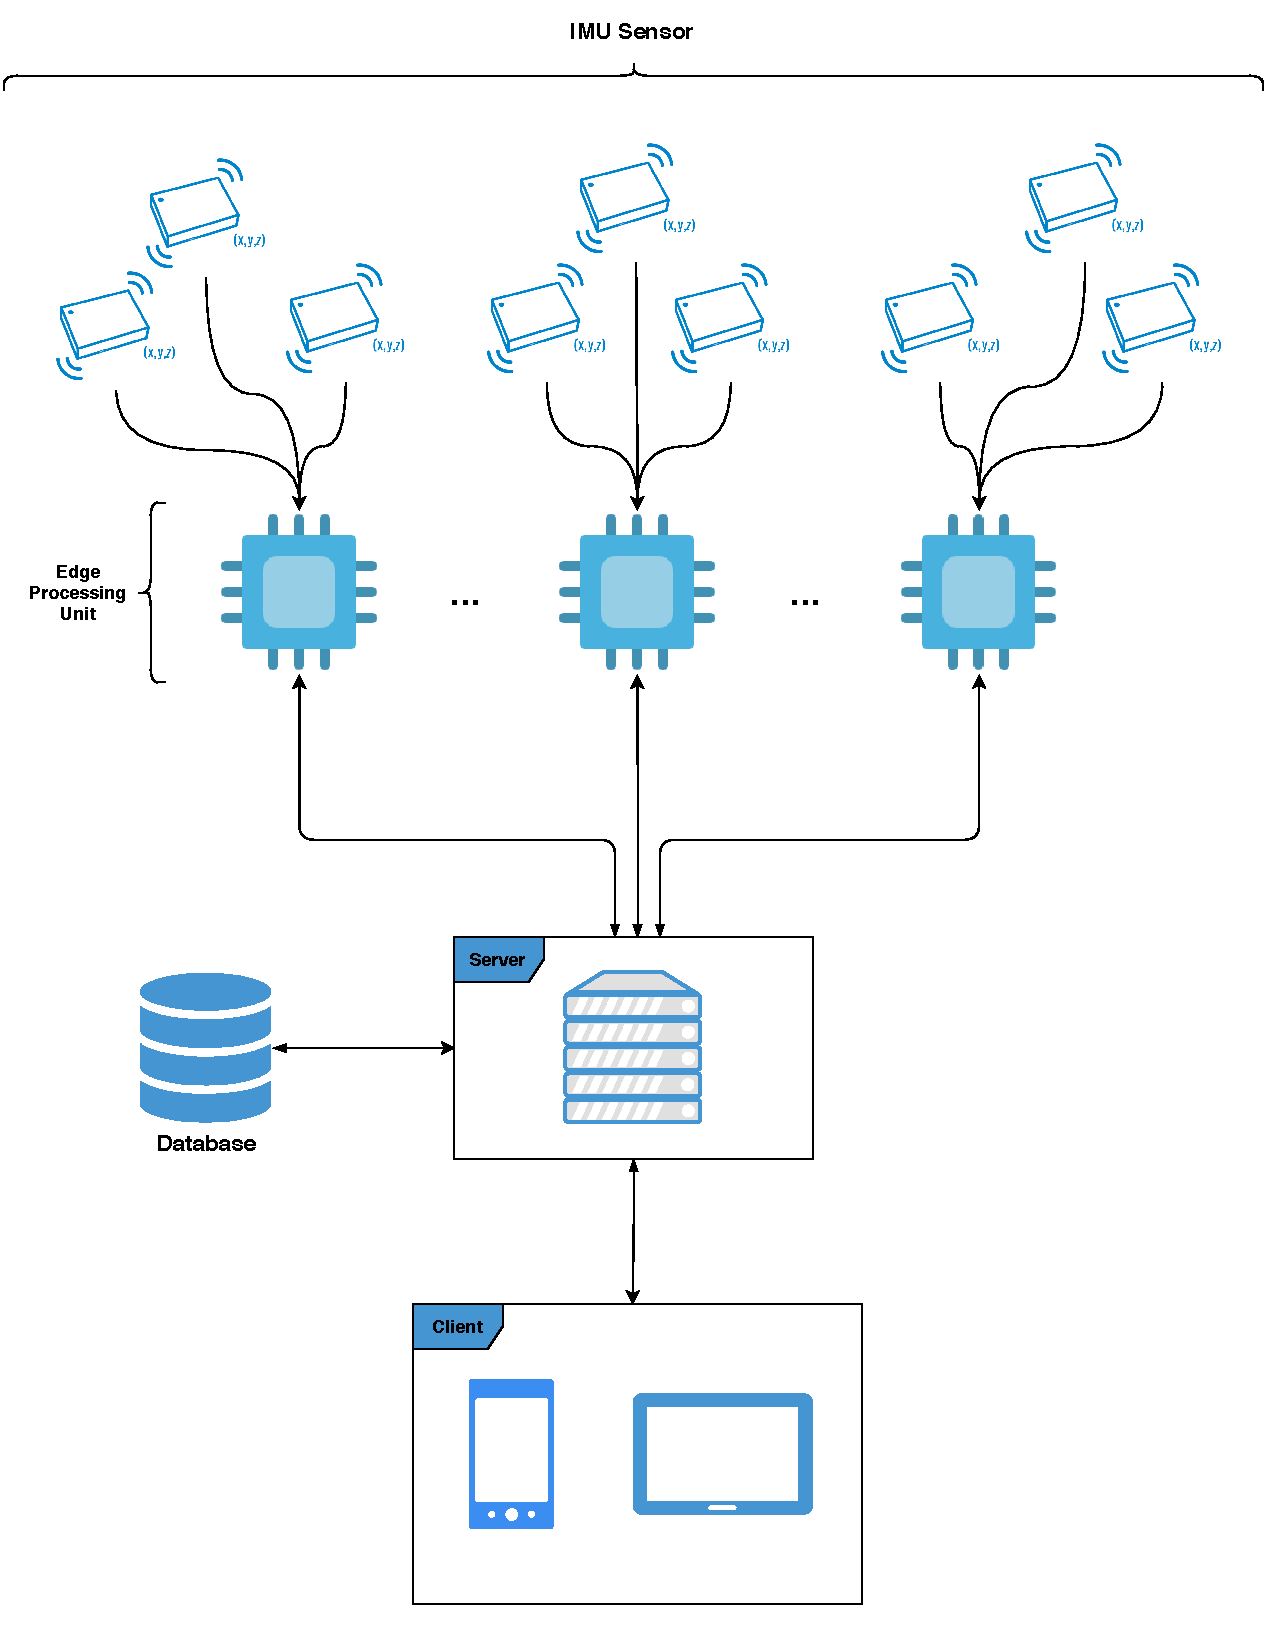
\includegraphics[width=.7\textwidth]{BLESportsTrackerArchitetureProposal.pdf}
    \caption{Proposed Architecture}
    \label{fig:architectureProposal}
\end{figure}

\subsection{Edge}
\label{subsec:edge}
The Edge segment is composed of at least one \gls{IMU} Sensor and one \gls{EPU}, that controls and receives information directly from the \gls{IMU} Sensor. The \gls{EPU} should also be capable of calculating insightful metrics, calculated with the raw data acquired from the \gls{IMU} Sensors.

\subsubsection{IMU Sensors}
\label{subsubsec:imu}
A \gls{IMU} Sensor is an integrated sensor package that measures a body's specific force, angular rate and orientation.

Specific force is a measurement of coordinate acceleration, which can be obtained by removing the gravitational acceleration.
It is measured with accelerometers.
Angular rate is the rate at which a body rotates, measured by gyroscopes.
Orientation is a description of how a body is placed in the place it occupies.
Using magnetometers, a body can be oriented relatively to the Earth's magnetic field.
%REFERENCE https://www.vectornav.com/support/library/imu-and-ins

For this application, IMU Sensors armed with 3-axis accelerometer and gyroscope should be used.

The \gls{IMU} sensors should attached to the player's body, in different locations (like the back, the foot or the hand), to track different metrics.


\subsubsection{Edge Processing Unit}
\label{subsubsec:epu}
The \gls{EPU} does the "hard work". Besides handling the connection and controlling the IMU Sensors operations, like starting and stopping the raw data collection, this unit has to collect the raw data sent by the IMU Sensors several times per second, and perform calculations with the gathered raw data to measure in-game metrics, which are then sent to the server, to be stored and shown to the User.


\subsection{Server}
\label{subsec:server}
The Server is the main piece of the architecture, allowing the interaction between the User and the IMU Sensors.

The Server can send instructions to the \gls{EPU}, controlling the \gls{IMU} Sensors operations.
When data is received from the \gls{EPU}, the Server stores it, so that it can be shown to the User, through the Client application.

The Server also hosts the Client Application, which communicates tightly with the Server.

\subsection{Client}
\label{subsec:client}
The Client Application provides the User an interface in which he can control and consult information about players, teams and games.

Indirectly he should trigger the start and stop of the data collection in the \gls{IMU} Sensors, which will then send the raw data to the \gls{EPU}. After the game metrics are calculated in the Edge, they are shown to the user, in the Client Interface.